\section{Application}
\label{sec:data}

We analyzed a dataset that was collected to investigate the feeding preferences of two species of wolf spider, Schizocosa ocreata and Schizocosa stridulans (Araneae: Lycosidae).  Every $6-12$ days, $10$ to $40$ spiders were hand-collected between October $2011$ and April $2013$ within Berea College Forest in Madison County, Kentucky, USA.  Spiders were removed from the litter using an aspirator, placed in separate $1.5$ mL microcentrifuge tubes filled with $95$\% EtOH, and preserved at $-20\celsius$ until DNA extraction.  In parallel, we also surveyed availability of forest floor prey using pitfall traps $(n = 32)$.  For the analysis, both species of Schizocosa were pooled and the number of spiders and prey were analyzed by month.  On average, $69$ spiders, $111$ Diptera, and $297$ Collembola were caught in each time period.  The range of the sample sizes across all $18$ months was $11$ to $181$ for caught spiders, $7$ to $322$ for trapped Diptera, and $101$ to $755$ for trapped Collembola.  Figure~\ref{fig:trapped} plots the total number of each order that was caught during each time period.

\begin{table}
  \label{tab:s1}
  \centering
  \begin{tabular}{llll}
    \hline
    \textbf{Target group} & \textbf{Primer names and sequences} $5'-3'$ & \textbf{Size (bp)} & \textbf{Source}\\
    \hline
    Collembola & Col3F: GGACGATYTTRTTRGTTCGT & 228 & \citet{Sint:2012} \\
    & Col-gen-A246: TTTCACCTCTAACGTCGCAG & & \\
    Diptera & DIPS16: CACTTGCTTCTTAAATrGACAAATT & 198 & \citet{Eitzinger:2014} \\
    & DIPA17: TTyATGTGAACAGTTTCAGTyCA &  & \\
  \end{tabular}
  \caption{Targeted prey orders, primer names and sequences, size of amplicon, and source of design for the detection of prey taxa within the guts of Schizocosa spiders.  Both primer sets were used in singleplex PCR assays.}
\end{table}

To determine whether spiders consumed dipterans and/or collemblans, we conducted a molecular analysis of their gut-contents.  First, DNA from spiders was extracted using Qiagen DNEasy\circledR Tissue Extraction Kit (Qiagen Inc., Chatsworth, California, USA) following the animal tissue protocol outlined by the manufacturer, with minor modifications.  Whole bodies of the spiders were first crushed to release prey DNA from within their alimentary canal for extraction.  The $200 \mu$L extractions were stored at $-20\celsius$ until PCR.  Second, order-specific primers from the literature were used to detect the DNA of Collembola and Diptera within the guts of the spiders.  Primer pairs designed by \citet{Sint:2012}, targeting the $18$S rDNA gene, were used to detect Collembola predation table~\ref{tab:s1}.  A PCR cycling protocol for $12.5 \mu$L reactions containing $1x$ Takara buffer (Takara Bio Inc., Shiga, Japan), $0.2$ mM dNTPs, $0.2 \mu$M of each primer, $0.625$ U Takara Ex TaqTM and $1.5 \mu$L of template DNA, using BioRad PTC$-200$ and C$1000$ thermal cyclers (Bio-Rad Laboratories, Hercules, California, USA), was optimized as follows: $95\celsius$ for $1$ minute, followed by $35$ cycles of $94\celsius$ for $30$ seconds, $61.2\celsius$ for $90$ seconds, and $72\celsius$ for $60$ seconds.  Primer pairs designed by \citet{Eitzinger:2014}, targeting the $18$S rDNA gene, were used to detect Diptera predation table~\ref{tab:s1}.  PCR cycling protocol for $12.5 \mu$L reactions with Takara reagents (as above) and $2 \mu$L of template DNA was optimized as follows: $95\celsius$ for $1$ minute, followed by $40$ cycles of $94$ for $45$ seconds, $60\celsius$ for $45$ seconds, and $72\celsius$ for $45$ seconds.  Both primer pairs were tested for cross-reactivity against a range of prey and predator species from the field site and in all cases, no amplification of DNA was observed, confirming suitable specificity of the primers for this study.  Lastly, electrophoresis of $10 \mu$L of each PCR product was later conducted to determine success of DNA amplification using $2\%$ Seakem agarose (Lonza, Rockland, Maine, USA) stained with $1x$ GelRed\texttrademark nucleic acid stain (Biotium, Hayward, California, USA).  This procedure allowed us to determine a presence or an absence of Diptera and Collembola DNA within each spider. 

\begin{figure}
  \centering
  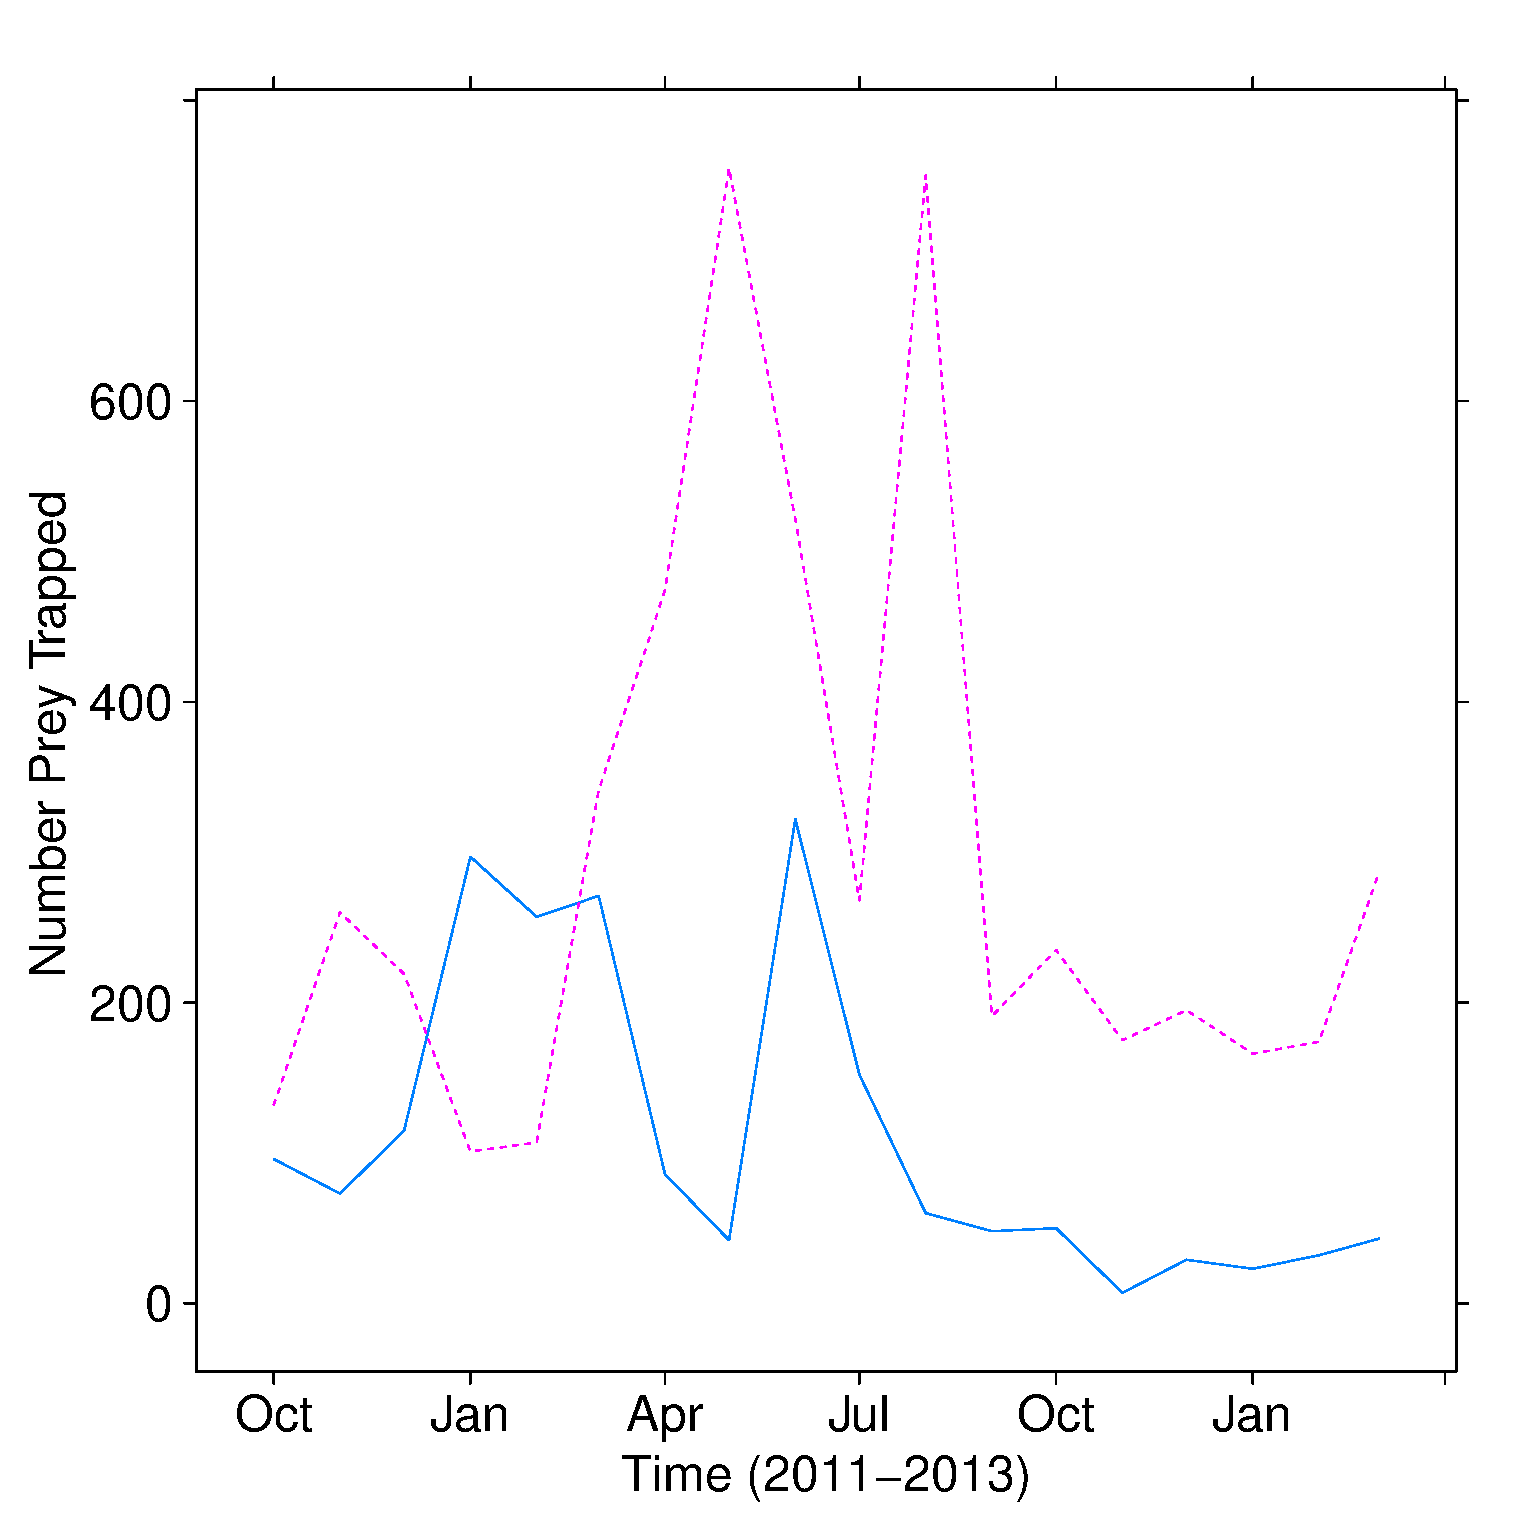
\includegraphics[scale=0.35]{prey_trapped}
  \caption{For both Collembola (pink/dashed) and Diptera (blue/solid), the plot shows the number of the prey trapped in each time period.}
  \label{fig:trapped}
\end{figure}

\begin{figure}
  \centering
  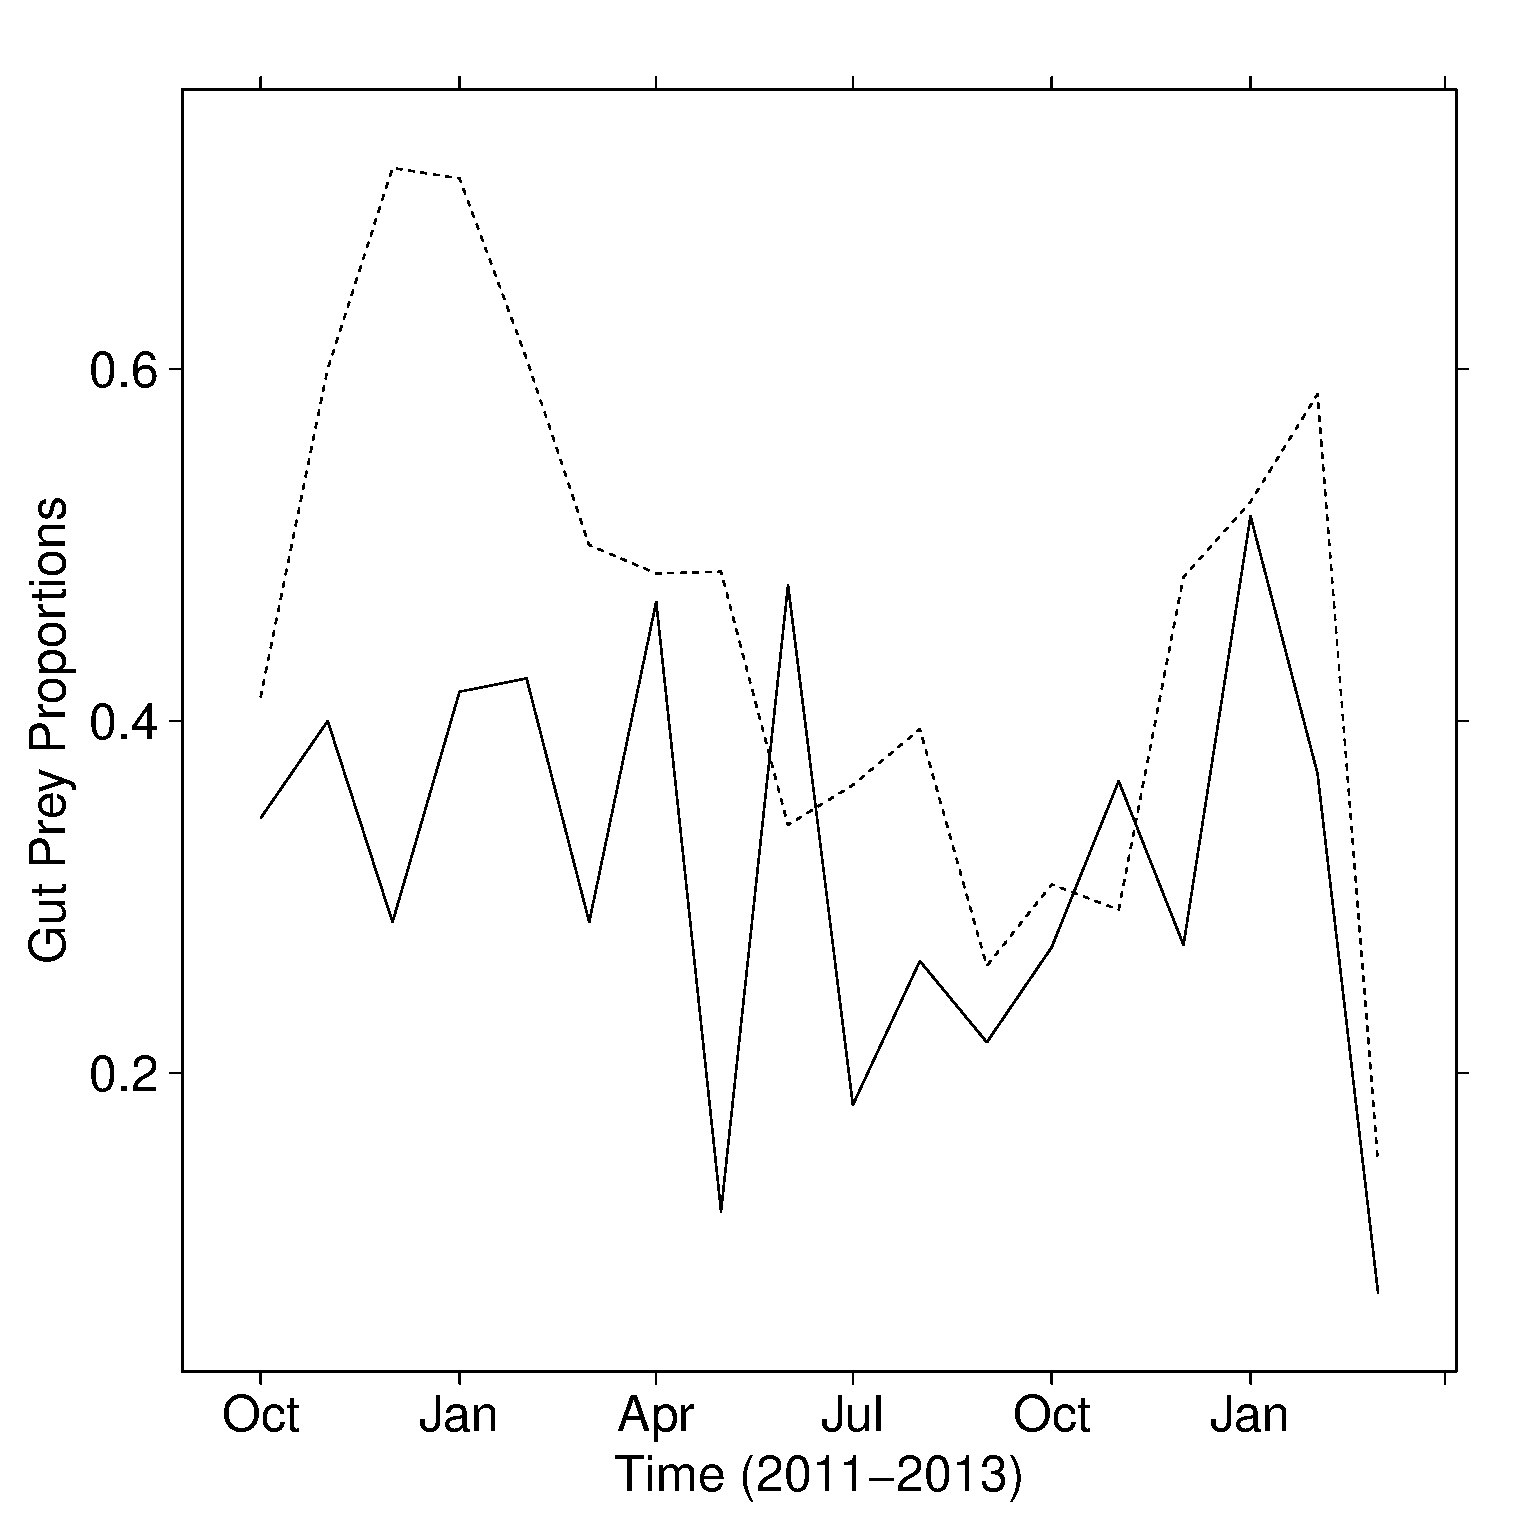
\includegraphics[scale=0.35]{prey_props}
  \caption{For both Collembola (pink/dashed) and Diptera (blue/solid), the plot shows the prey proportions in the sampled wolf spiders' guts in each time period.}
  \label{fig:props}
\end{figure}


These data provide an example of our hierarchy of hypotheses.  First, we tested model $c_{st} = c$ against $c_{st} = c_s$, to determine whether or not the wolf spider has different preferences for the two orders Diptera  and Collembola.  With, one degree of freedom, this likelihood ratio test indicated, $p-value < 0.0001$,  that two parameters, one for each order, fits these data better than one parameter for both.  Similarly, we tested whether or not there was a significant effect across time by testing model $c_{st} = c$ against $c_{st} = c_t$.  Here, the likelihood ratio test, with $17$ degrees of freedom, implies that the wolf spiders of the Berea College Forest eat these prey orders at different rates across the months of the year, $p-value < 0.0001$.  In fact, we find that the most parameter rich model, $\lambda_{st} = c_{st} \gamma_{st}$ fits these data better than is expected by chance, $p-value < 0.0001$.  Model $c_{st}$ estimates $72$ parameters in total; since, in this case, there are two prey of interest and $18$ time periods, it takes $36$ parameters to estimate each $c_{st}$ and $\gamma_{st}$.  Figures~\ref{fig:est_coll},~\ref{fig:est_dipt} plot the point estimates and $95\%$ confidence intervals of $c_{st}$, for both prey across all time periods.  

\begin{figure}
  \centering
  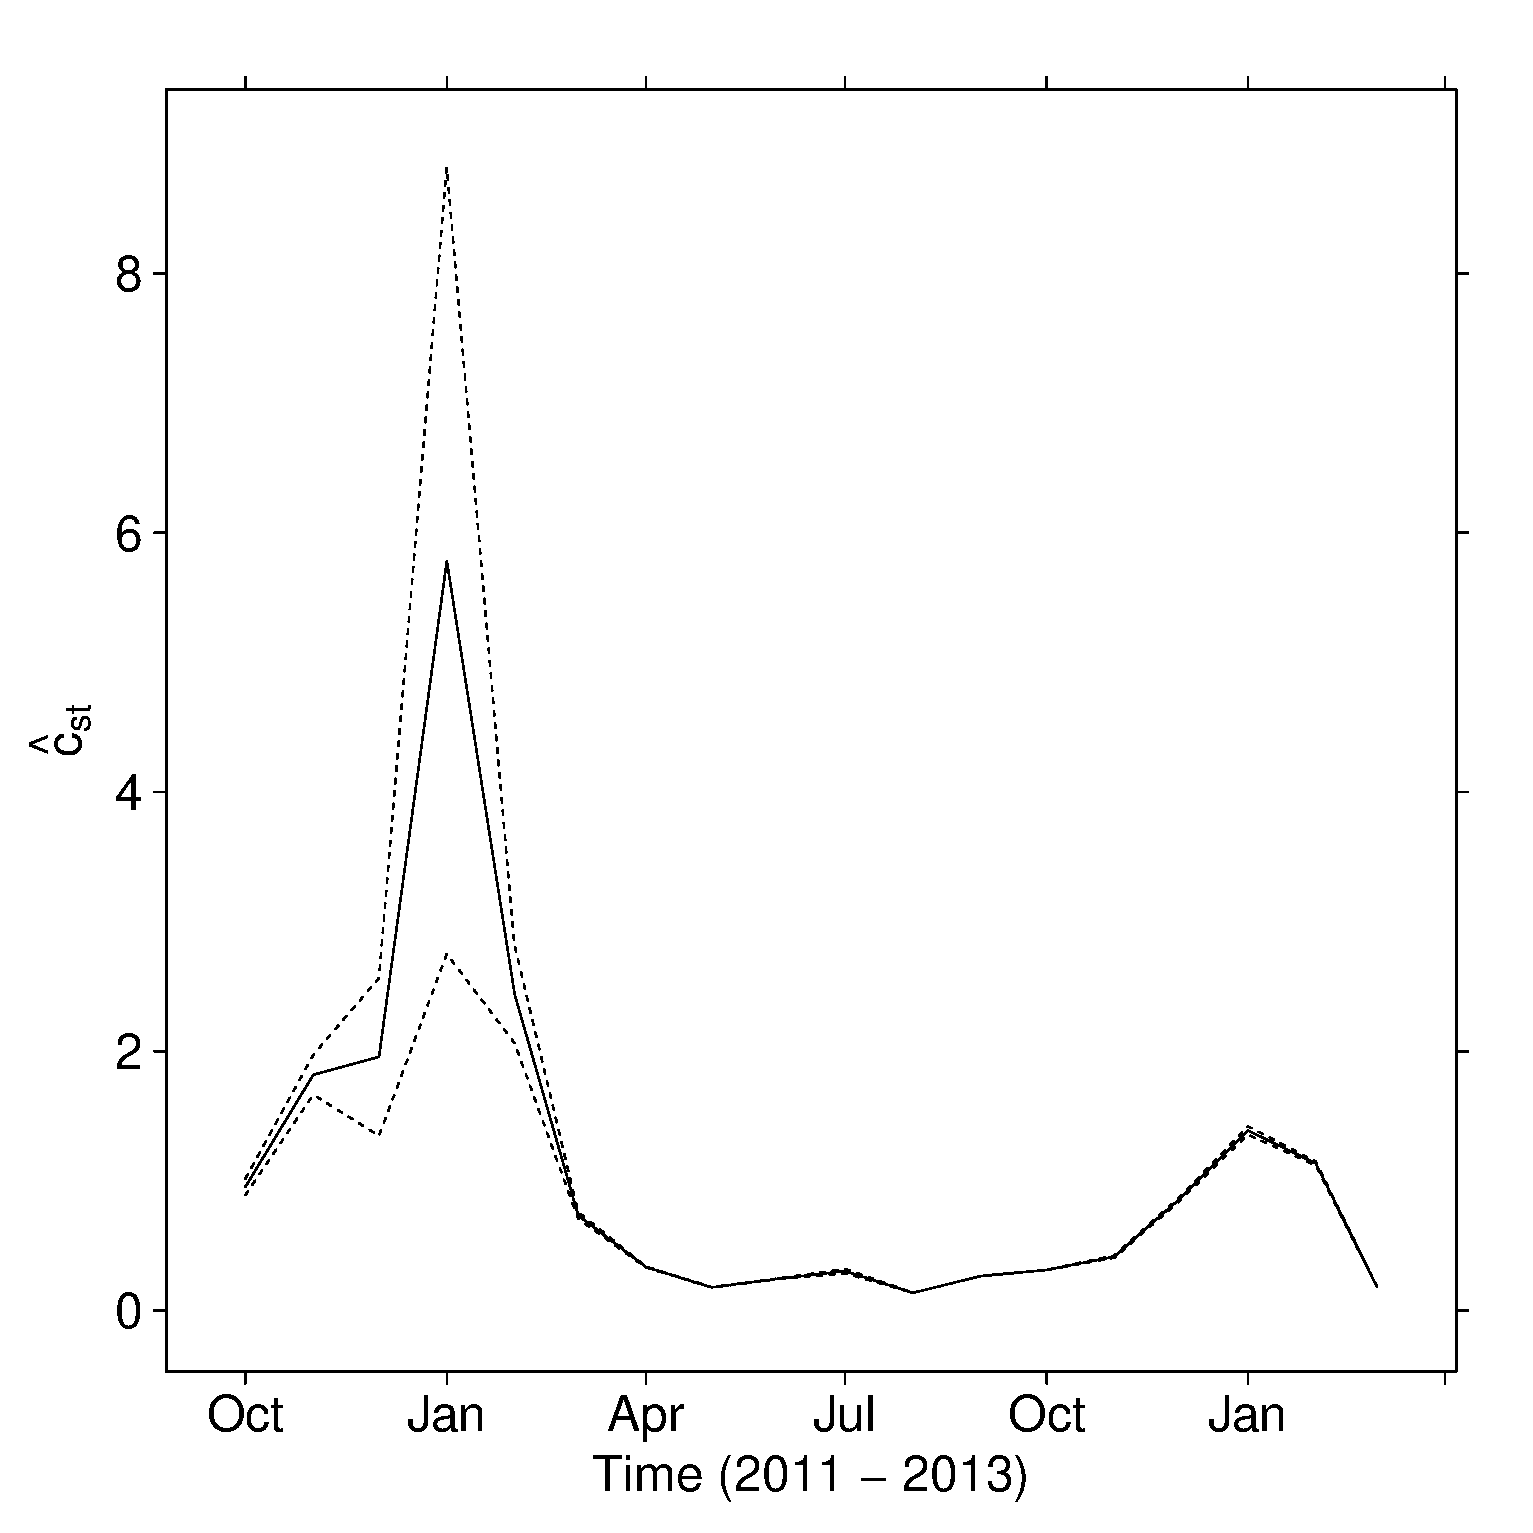
\includegraphics[scale=0.35]{est_coll}
  \caption{Point estimates (blue/solid) and $95\%$ confidence intervals (pink/dashed) as estimated from the model $c_{st}$ for Collembola.}
  \label{fig:est_coll}
\end{figure}

\begin{figure}
  \centering
  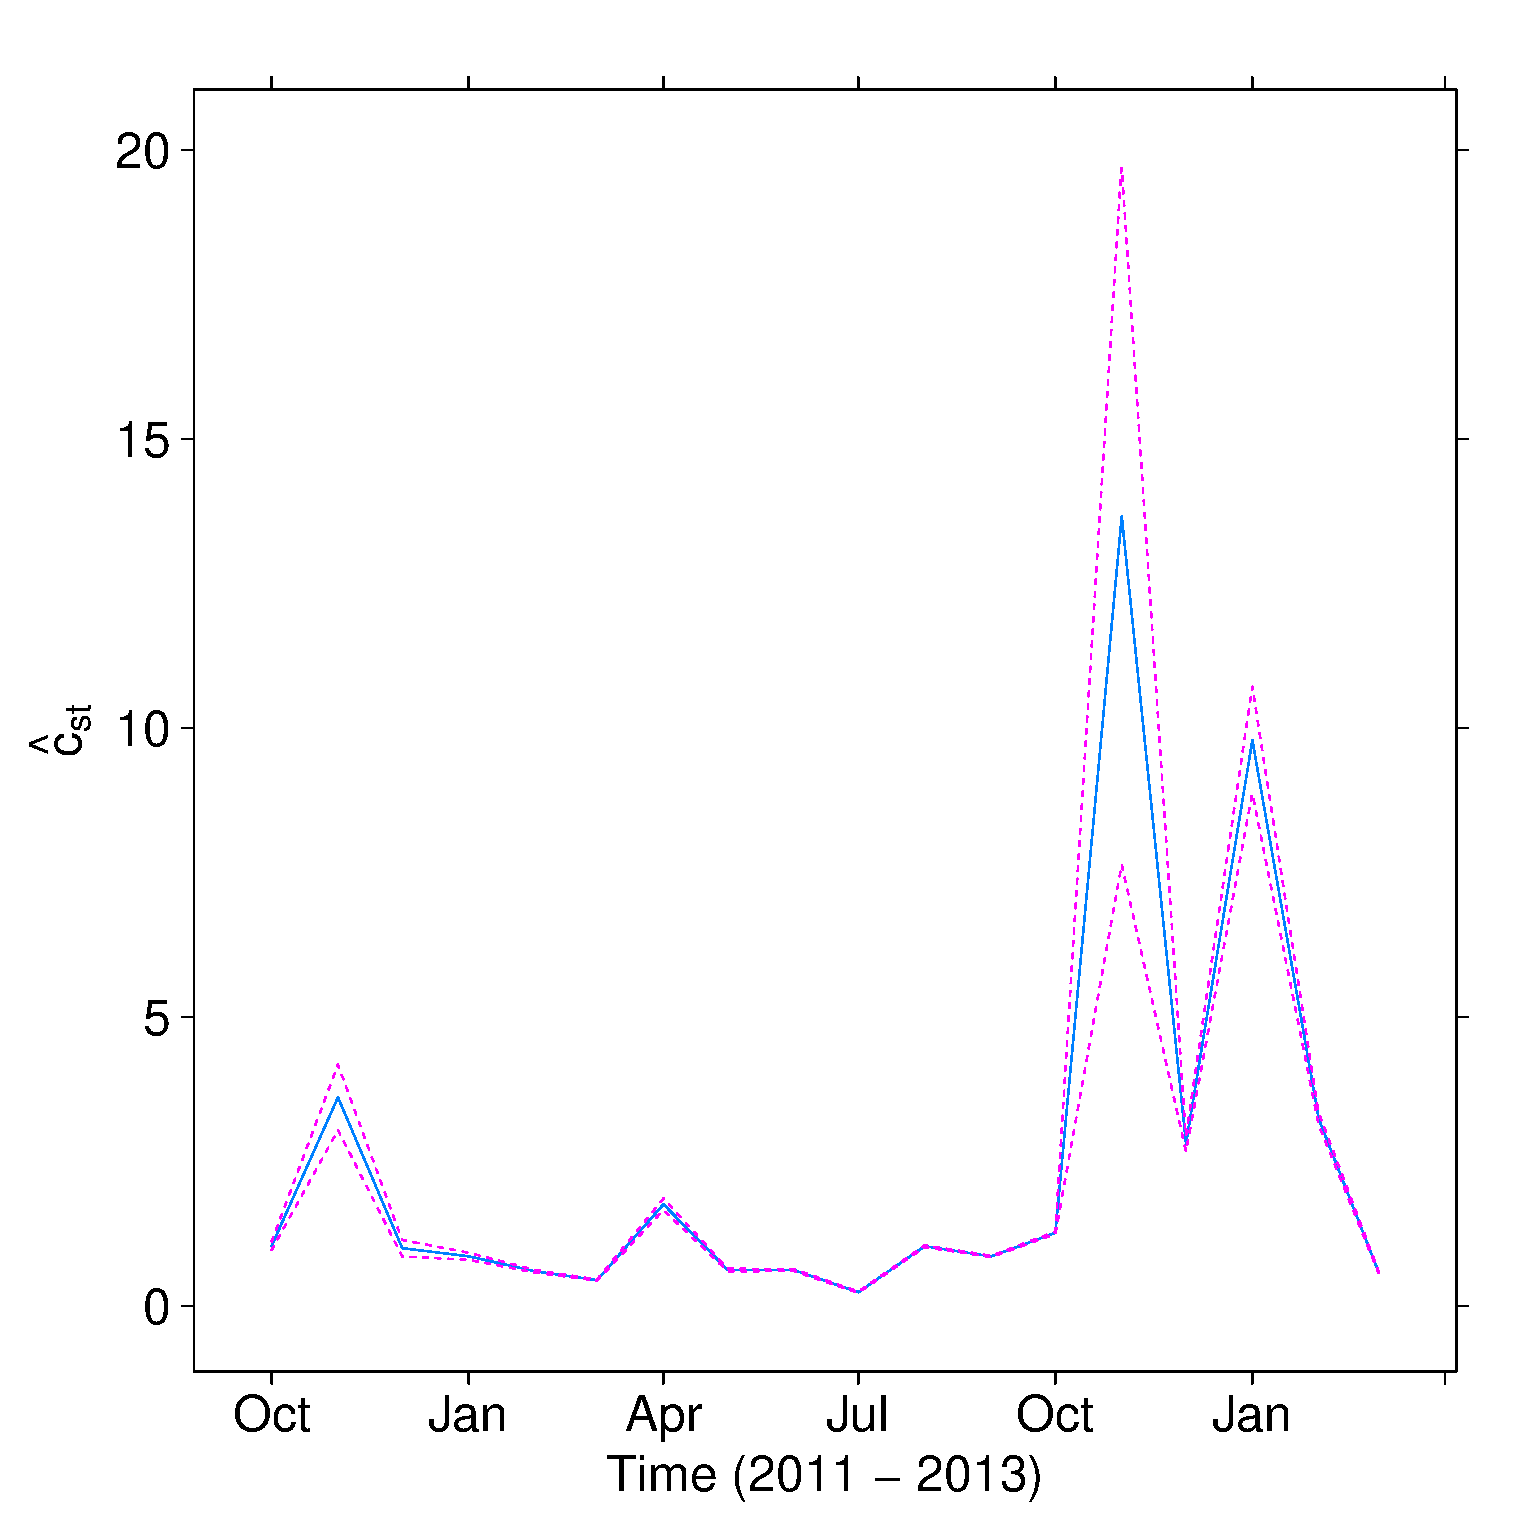
\includegraphics[scale=0.35]{est_dipt}
  \caption{Point estimates (blue/solid) and $95\%$ confidence intervals (pink/dashed) as estimated from the model $c_{st}$ for Diptera.}
  \label{fig:est_dipt}
\end{figure}

With point estimates of $c_{st}$ under the model $\lambda_{st} = c_{st} \gamma_{st}$, we can test any number of linear contrasts.  For instance, $c_{1t} = c_{2t}$, for $t \in \{1, \ldots, 18\}$.  Using a level of significance of $0.05$, and after making a Bonferroni multiple comparisons adjustment, the data can not say that the two prey are differently preferred in October, November, and December of $2011$ and for March and July of $2012$.  


%%% Local Variables: 
%%% mode: latex
%%% TeX-master: "main"
%%% End: 
